%%%%%%%%%%%%%%%%%%%%%%%%%%%%%%%%%%%%%%%%%%%%%%%%%%%%%%%%%%%%%%%%%%%%%%%%%%%
%%  chapter5.tex  –  Chapter 5: RobustIDPS.ai Software Platform
%%  v9 – Production deployment chapter: target users, 51-page PWA,
%%       10 functional groups, 17 models, LLM defence, PQC-IDS,
%%       Snort/Suricata plug-in, 8 figure placeholders for screenshots.
%%       Only \section headings go to TOC.
%%%%%%%%%%%%%%%%%%%%%%%%%%%%%%%%%%%%%%%%%%%%%%%%%%%%%%%%%%%%%%%%%%%%%%%%%%%

\chapter{Network Traffic Analysis System Based on the RobustIDPS.ai Software Platform}
\label{ch:platform}

This chapter systematically presents the software \emph{system}
\textsf{RobustIDPS.ai}~\cite{Anaedevha2026robustidps}
(DOI:~\url{10.5281/zenodo.19129512}; source code:
\url{https://github.com/rogerpanel/robustidps.ai}) that realises
the Hybrid~IDPS tuple of \S\ref{sec:hybrid_idps_math_model} for the
network-traffic-protection sector. The chapter follows the
three-part spine set out by the scientific supervisor's guidance:
\emph{(I)~problem statement}~--- the inputs, outputs, and operating
mode of the system for this sector are formalised
(\S\ref{sec:platform_problem_statement});
\emph{(II)~description of the system / software implementation}~---
the chapter systematically covers use cases, functionality,
documentation, frontend and backend implementation, the two-plane
architecture (Python control plane + Rust data plane, release~v4),
functional groups (51~pages across 10~groups), 17~integrated
detection models, the Rust edge-agent migration with the kernel-
resident XDP fast path, and operational deployment infrastructure
(\S\ref{ch:platform}--\S\ref{sec:deployment});
\emph{(III)~approbation of the system}~--- the chapter
systematically documents the benchmark validation results, the
comparison with commercial and open-source platforms, the
open-source contribution, and the letters of implementation from
the participating organisations
(\S\ref{sec:platform_comparison}--\S\ref{sec:opensource}).
At least six screenshots of the user interface are included to
illustrate the operational capabilities of the system.

The chapter offers an exhaustive description of the software
system as a direct instantiation of the mathematical model of the
Hybrid~IDPS formulated in Chapter~\ref{ch:methods}: each of the
seven methods (M1--M7) is mapped onto a concrete software
component with explicit APIs and operational metrics.
Architecturally, the platform follows security-by-design
principles, including a multi-tenant role-based access control
(RBAC) model, full audit logging of user actions through
structured logs, secure storage of sensitive configuration
parameters via integration with HashiCorp Vault, and a strict
segmentation between the control and data planes described in
\S\ref{sec:platform_problem_statement}. This approach yields
traceability from mathematical theorems to running code with the
minimal abstraction gap and enables independent developers and
security integrators to reproduce the claimed quality, robustness,
and efficiency figures on their own infrastructure. In addition
to the published source code (Zenodo,
DOI:~\url{10.5281/zenodo.19129512}), the platform ships with
complete technical documentation, demonstration datasets, and
automated test scenarios that lower the barrier to entry for
academic research groups and industrial cybersecurity teams.

%%=====================================================================\section{Problem Statement: Network Traffic Protection by the Hybrid~IDPS System}
\label{sec:platform_problem_statement}%%=====================================================================

The task of network traffic protection is treated in this chapter as
the concrete instantiated task of the Hybrid~IDPS tuple of
\S\ref{sec:hybrid_idps_math_model}. Formally, the system receives at
its input a stream of network packets (PCAP, NetFlow, EVE~JSON) and
signature-engine alerts (Snort, Suricata) aggregated by the
data-to-graph pipeline of Chapter~\ref{ch:adaptation}; at its
output the system produces ranked alerts, deployable Snort/Suricata
rules, and active-response control actions (flow blocking, node
isolation, SIEM/SOAR escalation). The high-level schematic is
shown in Fig.~\ref{fig:platform_problem_box}.

\textsf{RobustIDPS.ai} is a comprehensive, AI-native intrusion
detection and prevention platform comprising 51 interconnected
pages organised into 10 functional groups and integrating 17
machine-learning and deep-learning models for network-traffic
classification across 34 attack classes and 83 engineered
features. The platform addresses three limitations of existing
commercial alternatives (CrowdStrike Charlotte AI, SentinelOne
Purple AI, Microsoft Security Copilot, Google
Sec-Gemini~\cite{Smith2023}): proprietary single-vendor LLM
integration that prevents cross-provider benchmarking, the
absence of systematic adversarial-robustness evaluation, and the
lack of support for post-quantum cryptographic traffic analysis.
The target user roles span SOC analysts of Tiers~1--3,
cybersecurity engineers integrating the system into existing
signature contours, MLSecOps researchers benchmarking new
detection methods, AI developers extending the model registry,
and academic teams reproducing the published experiments.

\begin{figure}[htbp]
\centering
\begin{tikzpicture}[font=\scriptsize,
  inp/.style={draw,rounded corners=2pt,fill=blue!10,
    minimum width=3.0cm,minimum height=11mm,align=center,thick},
  sys/.style={draw,rounded corners=3pt,fill=orange!18,
    minimum width=5.0cm,minimum height=22mm,align=center,
    font=\small\bfseries,thick,draw=orange!70!black},
  outbx/.style={draw,rounded corners=2pt,fill=green!12,
    minimum width=3.0cm,minimum height=11mm,align=center,thick,
    draw=green!55!black},
  arr/.style={-{Stealth[length=2.5mm]},semithick,gray!75!black,thick}]
\node[inp] (in1) {Network packets\\stream / NetFlow};
\node[inp,below=4mm of in1] (in2) {Snort/Suricata\\signature alerts};
\node[sys,right=22mm of $(in1)!0.5!(in2)$] (sys)
  {Hybrid~IDPS\\system\\\textsf{RobustIDPS.ai}\\\scriptsize 17 Models M1--M7};
\node[outbx,right=22mm of sys.north east,yshift=0mm,anchor=west] (out1)
  {Ranked\\alerts};
\node[outbx,right=22mm of sys.east,anchor=west] (out2)
  {Snort/Suricata\\rules};
\node[outbx,right=22mm of sys.south east,anchor=west] (out3)
  {Active actions\\(SIEM/SOAR)};
\draw[arr] (in1) -- (sys.north west);
\draw[arr] (in2) -- (sys.south west);
\draw[arr] (sys.north east) -- (out1);
\draw[arr] (sys.east) -- (out2);
\draw[arr] (sys.south east) -- (out3);
\end{tikzpicture}
\caption{Problem statement for network traffic protection by the
Hybrid~IDPS system in the \textsf{RobustIDPS.ai} implementation.
Left~--- input streams (network packets, NetFlow, signature-engine
alerts); centre~--- the system with 17~integrated Models M1--M7;
right~--- output artefacts (ranked alerts, deployable
Snort/Suricata rules, control actions for SIEM/SOAR orchestration).}
\label{fig:platform_problem_box}
\end{figure}

\noindent\textbf{Target users of the system.} The platform
serves five categories of users. \emph{SOC Analysts (Tiers~1--3)}~---
security-operations-centre personnel who monitor, investigate, and
respond to security incidents; the platform provides agentic
auto-investigation, natural-language threat hunting, automated
incident reporting, and uncertainty-driven alert triage that
reduces mean triage time by 34\%. \emph{Cybersecurity engineers}~---
network-security professionals who deploy and configure intrusion
detection systems; the platform generates deployable Snort/Suricata
rules from detected threats and provides real-time monitoring
through WebSocket-based streaming. \emph{MLSecOps researchers}~---
machine-learning security researchers who evaluate the robustness
of AI components; the platform provides integrated adversarial
testing (six attack families), LLM attack-surface evaluation
(five modules), and MLSecOps compliance dashboards (MITRE ATT\&CK,
OWASP LLM Top~10, NIST AI RMF). \emph{AI developers}~---
researchers and engineers building graph-based detection models;
the platform exposes 17 pre-trained models with configurable
hyperparameters, an ablation studio, and reproducible benchmarking
datasets. \emph{Academic researchers}~--- PhD students,
postdoctoral fellows, and faculty conducting research on
graph-neural-network robustness; the platform serves as a
reproducible research instrument with DOI-archived code and
datasets.

\noindent\textbf{Implementation technology stack.}
RobustIDPS.ai is deployed as a Progressive Web Application (PWA)
with the following technology stack. \emph{Frontend}~--- a
React~18 single-page application with Material-UI components,
responsive design, and PWA manifest for offline-capable deployment
with service-worker caching. \emph{Backend}~--- a Flask/Python
3.11+ backend with 60+ RESTful API endpoints, persistent WebSocket
channels for real-time monitoring, and Celery for asynchronous
task execution (model training, batch analysis). \emph{Data
layer}~--- PostgreSQL~16 for relational persistence (user
profiles, detection logs, investigation records), Redis~7 for
caching and session management, and file-system storage for
uploaded PCAP/CSV datasets. \emph{Orchestration}~--- Docker
Compose enables single-command deployment with environment-based
configuration for development, staging, and production profiles.

\noindent\textbf{Two-plane architecture (release v4).} Release~v4
introduces a strict separation between the Python \emph{control
plane} and the Rust \emph{data plane}. The control plane hosts the
RESTful API, the WebSocket-streaming layer, the SOC-Copilot
analytics, and the model registry; the data plane hosts the
high-throughput Rust edge agent, the kernel-resident XDP fast
path, and the in-memory model-update channel. The two planes
communicate through gRPC over a mutually authenticated TLS
channel; the data plane never accepts user-facing HTTP traffic and
exposes no public ports. This separation provides three concrete
benefits: \emph{(i)~security}, since the kernel-attached components
sit behind a dedicated trust boundary; \emph{(ii)~independent
scalability}, since the control plane and the data plane scale
along orthogonal dimensions (number of analysts vs.\ wire-speed
throughput); and \emph{(iii)~clean upgrade path}, since the
existing 51 frontend pages are preserved untouched as the data
plane evolves toward INT8-distilled student models and
kernel-resident fast paths.

\noindent\textbf{Target properties of the system in this sector.}
The solution to the network-traffic-protection task by the
\textsf{RobustIDPS.ai} system systematically satisfies four of the
six properties P1--P6 from \S\ref{subsec:six_properties}:
\emph{P1} (adversarial resilience, eq.~\eqref{eq:adv_resilient_property})
through the integration of Models~M1, M4, and~M7;
\emph{P2} (robustness, eq.~\eqref{eq:robustness_property})
supported by the benchmark results of
Chapter~\ref{ch:adaptation}~(\S\ref{sec:method_results});
\emph{P3} (efficiency, eq.~\eqref{eq:efficiency_property})
provided by the v4 two-plane architecture with the kernel-resident
XDP fast path (\S\ref{ch:platform}); and
\emph{P5} (human factor, eq.~\eqref{eq:calibration_property})
realised through uncertainty-guided alert triage in the SOC
copilot (\S\ref{ch:platform}).

\noindent\textbf{AI Active Defence.} The AI Active Defence group
contains five pages supporting proactive cybersecurity scenarios.
\emph{Red-Team Arena} provides an interactive environment for
running adversarial attacks against the deployed detection models
under six attack families (FGSM, PGD, C\&W, DeepFool, HopSkipJump,
BoundaryAttack), allowing researchers and red-team testers to
verify the robustness of their trained models before deployment.
\emph{Threat Response} automates the generation of control actions
through integration with SOAR systems (Phantom, Demisto, IBM
Resilient). \emph{SOC Copilot} (a multi-provider, open-source
successor to Microsoft Security Copilot) provides
epistemically-guided alert triage based on the UC-HGP module of
Method~M6. \emph{Federated Learning} implements Byzantine-resilient
aggregation (FedLLM-API of Method~M2) with support for up to 50
participants and formal
$(\varepsilon{=}0.85,\delta{=}10^{-5})$-differential privacy.
\emph{Attack-Chain Predictor} forecasts the most probable next
steps of an attacker from observed early indicators of compromise
using the game-theoretic certification of Method~M7.

\noindent\textbf{LLM Attack Surfaces.} Six pages of this group
systematically cover the attack surfaces against deployed LLM
components inside security infrastructure~--- a domain not
covered by any existing commercial platform. Beyond the five
modules described above (prompt injection, jailbreaks, RAG
poisoning, multi-agent chain, data poisoning), a sixth page~---
\textsf{MambaGuard}~--- presents a protocol-aware detector for
four LLM-agent protocols: MCP (Model Context Protocol from
Anthropic), ACP (Agent Communication Protocol from Google), A2A
(Agent-to-Agent Protocol from Microsoft), and ANP (Agentic
Network Protocol). \textsf{MambaGuard} achieves macro-averaged
F1=0.978 on the in-house MambaGuard-bench dataset at an inference
time of 1.8\,ms/flow. The defence-ensemble certification combines
randomised smoothing for continuous perturbation budgets, a
conformal Bayesian interval for calibration of probabilistic
outputs, and a regret certificate for online agentic scenarios.
The group is also integrated with the OWASP LLM Top~10 (2025)
compliance dashboard with automatic mapping of every detection
into the corresponding risk category.

\noindent\textbf{AI Command Centre.} The AI Command Centre is the
primary operational interface and includes five pages for
end-to-end traffic analysis from upload to alert resolution. The
\emph{Main Dashboard} renders real-time detection statistics:
total number of analysed flows, distribution of attacks across
categories, model-accuracy metrics, and severity-based alert
breakdown; interactive time-series charts show detection trends
over configurable windows (from 1~hour to 30~days). The
\emph{Upload and Analyse} page accepts PCAP or CSV files via
drag-and-drop; the \texttt{FeatureExtractor} module computes the
83-dimensional feature vector from raw packet data, applies
z-standardisation, and routes the features to the selected
detection model. \emph{Live Monitor} provides WebSocket-based
real-time streaming with a configurable retention window and
sub-second push notifications for high-severity alerts;
simultaneous display of outputs from multiple models is supported
for ensemble comparison. The \emph{Alert Causality} page builds
graphs of temporal dependencies between related alerts, allowing
analysts to trace multi-stage attack campaigns; correlation is
based on shared source/destination IPs, temporal proximity
($\pm$30\,s), and MITRE ATT\&CK~\cite{Hernandez2015} technique
links.

\noindent\textbf{Registry of Functional Groups.} The 51 pages of
the platform are organised into ten functional groups providing
an end-to-end detection-and-response cycle: \emph{(1)~AI Command
Centre} (5~pages); \emph{(2)~AI Active Defence} (5); \emph{(3)~SOC
Intelligence Suite} (6); \emph{(4)~LLM Attack Surfaces} (6);
\emph{(5)~MLSecOps Standards} (3); \emph{(6)~AI Security and
Governance} (4); \emph{(7)~AI Novel Methods} (7); \emph{(8)~AI
Data and Models} (4); \emph{(9)~Operations and Deployment} (6);
and \emph{(10)~System} (5). The platform integrates more than 13
neural-network architectures implementing all seven methods
(M1--M7) of Chapter~\ref{ch:methods}, including three new
detectors introduced in release~v4: \textsf{MambaGuard}
(selective state-space model with a three-tier certification
system), \textsf{SODE-Guard} (It\^o stochastic differential
equation with an anti-concentration robustness certificate in the
style of~\cite{Cohen2019}), and \textsf{SSL-GraphAnomaly Full}
(a self-supervised six-component architecture for anomaly
detection without labelled attack samples).

\noindent\textbf{Operational Deployment Infrastructure.}
Release~v4 ships with a production-grade deployment toolkit
organised into three layers: \texttt{systemd} units for
bare-metal operation (with a capability-minimised environment
combining \texttt{CAP\_NET\_RAW}, \texttt{CAP\_NET\_ADMIN},
\texttt{CAP\_BPF}, \texttt{CAP\_PERFMON} with
\texttt{NoNewPrivileges}, \texttt{ProtectSystem=full}, and
\texttt{PrivateTmp}); a multi-stage \texttt{Dockerfile} for
container smoke testing and portability (two-stage build with a
runtime image of $\sim$120\,MiB, supporting both \texttt{amd64}
and \texttt{arm64} via \texttt{TARGETARCH}); and the
distil-and-push automation orchestrated by \texttt{cron} through
the \texttt{distill\_and\_push.py} script ($\sim$270 lines),
which performs the full cycle: retraining of the INT8 ONNX
student from the current \textsf{SurrogateIDS} teacher weights,
artefact verification, SHA-256 computation, fan-out delivery via
\texttt{EdgeFleet.push\_model()}, activation confirmation through
\texttt{gather\_stats}, and a single JSON-line log per run in
\texttt{/var/log/robustidps/distill\_and\_push.jsonl}.

%%=====================================================================
%%   PART II: DESCRIPTION OF THE SYSTEM / SOFTWARE IMPLEMENTATION
%%   (systematically covered in \S\S5.2--5.12 below: use cases,
%%    functionality, documentation, frontend/backend, architecture,
%%    models, deployment)
%%=====================================================================

%%=====================================================================\section{Rust Edge-Agent Migration and the XDP Fast Path}
\label{sec:rust_edge_agent}%%=====================================================================

Release v4 introduces a native \emph{Rust edge agent} into the
platform's data plane, enabling traffic decisions at
\emph{wire speed}. The migration is structured as six step-wise
crates and does not touch the existing user interface.

\noindent\textbf{Step 1: \texttt{agent-features}}~--- a pure-Rust
implementation of the 83-dimensional flow feature vector
extraction from PCAP, bit-for-bit consistent with the reference
Python implementation (validated on 1\,M flows of CIC-IoT-2023).

\noindent\textbf{Step 2: \texttt{agent-netfilter}}~--- atomic
application of block-list rules through an \texttt{nftables} binding
using a two-phase commit/rollback mechanism that eliminates
inconsistency windows.

\noindent\textbf{Step 3: \texttt{agent-edge}}~--- a long-running
gRPC daemon with hot-swap of ONNX models behind a \texttt{RwLock}
and server-streaming of flow records to the control plane.

\noindent\textbf{Step 4: \texttt{agent-inference}}~--- an INT8 ONNX
student model distilled from the \textsf{M1}--\textsf{M7} teacher
ensemble. Achieves 0.18\,ms/flow latency on a single Intel Xeon
Gold~6248 core with less than 0.9~p.p.~F1 loss against the teacher.

\noindent\textbf{Step 5: \texttt{agent-xdp}}~--- in-kernel LPM-trie
block list attached through the XDP hook in \texttt{Native} mode on
\texttt{eth0}. Packets from confirmed malicious prefixes are dropped
\emph{before} \texttt{sk\_buff} allocation, yielding microsecond-scale
decisions.

\noindent\textbf{Step 6: online model update channel}~--- the
\texttt{ApplyModelUpdate} gRPC method chunks the model into 3-MiB
blocks with SHA-256 integrity verification, enabling atomic
replacement of the running ONNX model without agent restart and
without dropping flows.

A summary of the performance figures is given in
Table~\ref{tab:rust_edge_perf}.

\begin{table}[H]
\centering
\caption{Performance of the Rust data plane (release v4) relative to
the reference Python implementation of release v3.}
\label{tab:rust_edge_perf}
\small
\setlength{\tabcolsep}{4pt}
\renewcommand{\arraystretch}{1.15}
\renewcommand{\arraystretch}{0.92}\begin{tabular}{@{}lrrr@{}}
\toprule
\textbf{Metric} & \textbf{v3 (Python)} & \textbf{v4 (Rust + XDP)} & \textbf{Gain}\\
\midrule
Inference latency (per-flow), ms      & 1.2     & 0.18    & $\times$6.7\\
Throughput, flows/s                   & 870\,K  & 5.8\,M  & $\times$6.7\\
Drop-decision latency, $\mu$s         & ---     & 4.1     & ---\\
RSS memory usage, MiB                 & 612     & 78      & $\times$7.8\\
Cold start to ready, s                & 9.4     & 0.7     & $\times$13\\
\bottomrule
\end{tabular}\end{table}

%%=====================================================================\section{Integration of the System with Existing Information-Security Tooling}
\label{sec:deployment}%%=====================================================================

RobustIDPS.ai is designed for deployment as a plug-in for existing intrusion detection frameworks, specifically Snort~3~\cite{Roesch1999} and Suricata. The architectural goal of integration is to preserve the organisation's prior investments in the signature contour and to augment it with an ML-native layer without requiring replacement of existing tools. This reduces implementation costs, simplifies internal audits, and ensures backward compatibility with existing incident-response procedures. The integration operates through two mechanisms:

\noindent\textbf{Rule Generation.} The IDS Rule Generator translates detected threats into deployable Suricata/Snort rules using 21 templates, enabling the ML-based detection to produce actionable outputs in the formats that existing infrastructure already consumes.

\noindent\textbf{Alert Feed Consumption.} The platform consumes Suricata/Snort alert logs (EVE JSON or unified2 format) as additional input, correlating signature-based detections with anomaly-based GNN classifications to reduce false positives and provide contextual enrichment.

Docker Compose orchestration enables single-command deployment. A \texttt{fast\_mode} toggle reduces inference latency by 60\% (disabling MC dropout and uncertainty quantification), achieving throughput exceeding 12,000 flows/second on a single CPU core --- sufficient for real-time analysis of 10\,Gbps links with appropriate parallelisation.

A minimal programmatic example of integrating the
\textsf{RobustIDPS.ai} system with Suricata through the REST~API is
given in Listing~\ref{lst:ridps_api}~--- the full cycle from a PCAP
file to generated Suricata rules fits into a few lines of client
code. Analogous integration templates are available for Snort~3
(via the \texttt{u2spewfoo} submodule for unified2 format
conversion), for AWS cloud environments (via \texttt{VPC Flow
Logs} and a connector to \texttt{Amazon GuardDuty}), and for
Microsoft Azure (via \texttt{NSG Flow Logs} and integration with
\texttt{Microsoft Sentinel}). All examples are available in the
official platform repository under the \texttt{integrations/}
directory together with ready-to-use Docker compositions for
reproducible test deployments.

\begin{lstlisting}[language=Python,caption={Integration of the \textsf{RobustIDPS.ai} system with Suricata through the REST~API (excerpt from \texttt{robustidps\_client.py}).},
label={lst:ridps_api},basicstyle=\ttfamily\footnotesize,
keywordstyle=\bfseries,commentstyle=\itshape\color{gray!60!black},
breaklines=true,frame=single,numbers=left,numberstyle=\tiny]
import requests

# 1. Submit a PCAP file to the Hybrid IDPS system for analysis
files     = {"pcap": open("traffic.pcap", "rb")}
params    = {"model": "surrogate", "fast_mode": False}
resp      = requests.post(
    "https://robustidps.local/api/v1/analyze",
    files=files, params=params, timeout=60,
).json()

# 2. Inspect per-flow detections with calibrated uncertainty
for flow in resp["flows"]:
    if flow["epistemic_uncertainty"] > 0.30:
        print(f"[TRIAGE] flow {flow['id']} -> analyst (uncertainty {flow['epistemic_uncertainty']:.2f})")
    elif flow["attack_class"] != "Benign":
        print(f"[ALERT] {flow['attack_class']} (conf {flow['confidence']:.2f}, MITRE {flow['mitre_techniques']})")

# 3. Push the generated Suricata rules back into the IPS
rules = requests.get("https://robustidps.local/api/v1/rules/suricata").text
with open("/etc/suricata/rules/robustidps.rules", "w") as f:
    f.write(rules)
requests.post("https://suricata.local/api/reload")
\end{lstlisting}

%%=====================================================================
%%   PART III: APPROBATION OF THE SYSTEM
%%   (systematically documents the benchmark validation results, the
%%    comparison with commercial and open-source platforms, the
%%    open-source contribution, and the letters of implementation
%%    from the participating organisations)
%%====

\paragraph{Bridge with the above.}Sections~\ref{ch:platform}--\ref{sec:deployment} above
have systematically realised the software \emph{system}
\textsf{RobustIDPS.ai} as the instantiation of Hybrid~IDPS for the
network-traffic-protection sector. The following
sections~\ref{sec:platform_comparison}--\ref{sec:opensource}
constitute the approbation part of the chapter and systematically
answer three questions:
\emph{(a)~how does the \textsf{RobustIDPS.ai} system compare with
commercial and open-source platforms of the same class
(CrowdStrike Charlotte AI, SentinelOne Purple AI, Microsoft
Security Copilot, Google Sec-Gemini, Snort~3, Suricata)};
\emph{(b)~what are the quantitative results of the systematic
validation of the system on the benchmark datasets and which
properties P1--P6 they support}; and
\emph{(c)~how is the system deployed and used in real industry
organisations, as evidenced by implementation acts received from
NII~IKT LLC (Novosibirsk) and Ksyrix LLC (Moscow); the act from
the Artificial Intelligence Center of NRNU MEPhI, Moscow, is in
the course of formalisation}.

%%=====================================================================\section{Comparison with Commercial and Open-Source Platforms}
\label{sec:platform_comparison}%%=====================================================================

The comparison of \textsf{RobustIDPS.ai} capabilities against
leading open-source and commercial platforms is performed along
nine key characteristics covering both functional detection
capabilities and architectural extensibility properties. The
systematic positioning analysis answers three important questions
for both the research and the industrial audience: \emph{(a)~what
are the technological advantages of the developed platform over
existing solutions?}; \emph{(b)~what is its contribution to the
open-source cybersecurity ecosystem?}; \emph{(c)~under which
operational scenarios does integrating \textsf{RobustIDPS.ai}
with existing open and commercial solutions deliver the best
organisational and economic outcome?} Open-source platforms
(\textsf{Snort 3}, \textsf{Suricata}) provide mature
signature-based detection and broad rule support, but lack
ML-based components, formal adversarial-robustness guarantees,
and large-language-model attack testing. Commercial platforms
(\textsf{CrowdStrike Falcon} with the \textsf{Charlotte AI}
module, \textsf{Microsoft Security Copilot}) provide AI-augmented
detection and automated response, but are closed-source, tied to
a single proprietary LLM vendor, do not support cross-provider
benchmarking, do not publish formal adversarial-robustness
certificates, and do not support post-quantum cryptographic
traffic. \textsf{RobustIDPS.ai} occupies a unique niche as the
only open platform that systematically covers all nine
characteristics listed in
Table~\ref{tab:platform_comparison}~--- from ML-based detection
with 17 models to post-quantum IDS and a NIST AI~RMF
dashboard~--- while providing reproducible research-grade
testing.

\begin{table}[htbp]\centering\small
\caption{Feature comparison with open-source and commercial platforms.}
\label{tab:platform_comparison}
\footnotesize
\renewcommand{\arraystretch}{0.92}\begin{tabular}{p{3.5cm}ccccc}
\toprule
\textbf{Capability} & \rotatebox{70}{\textbf{RobustIDPS.ai}} & \rotatebox{70}{\textbf{Suricata}} & \rotatebox{70}{\textbf{Snort 3}} & \rotatebox{70}{\textbf{CrowdStrike}} & \rotatebox{70}{\textbf{MS Copilot}} \\
\midrule
ML detection (17 models)  & \checkmark & ---        & ---        & Partial    & ---        \\
Adversarial robustness      & \checkmark & ---        & ---        & ---        & ---        \\
Continual learning          & \checkmark & ---        & ---        & ---        & ---        \\
Multi-provider LLM          & \checkmark & ---        & ---        & Proprietary& Proprietary\\
LLM attack testing          & \checkmark & ---        & ---        & ---        & ---        \\
MITRE ATT\&CK~\cite{Hernandez2015}      & \checkmark & Partial    & Partial    & \checkmark & \checkmark \\
NIST AI RMF dashboard       & \checkmark & ---        & ---        & ---        & ---        \\
Post-quantum IDS            & \checkmark & ---        & ---        & ---        & ---        \\
Open-source                 & \checkmark & \checkmark & \checkmark & ---        & ---        \\
\bottomrule
\end{tabular}\end{table}

%%=====================================================================\section{Analysis of Operational Characteristics of the System}
\label{sec:platform_validation}%%=====================================================================

\subsection{Model Performance}

All 17 models are validated on the CIC-IoT-2023 benchmark (Table~\ref{ch:platform}). The SurrogateIDS ensemble achieves the highest accuracy (97.8\%) through its seven-branch architecture. MambaShield delivers competitive accuracy (95.9\%) at the lowest latency (0.5\,ms), making it the preferred choice for deployments with high throughput requirements. CyberSecLLM achieves the lowest ECE (0.025) thanks to the calibration properties of language-model probability outputs. CT-TGNN provides 98.3\% accuracy with 47\,ms median inference latency and 8.7~million events per second throughput, with per-category recall of 99.1\% for DDoS, 96.8\% for reconnaissance, 97.3\% for web attacks, 98.6\% for brute force, 95.2\% for spoofing, 98.9\% for malware, and 97.4\% for Mirai. The SDE-TGNN extension adds a stochastic-diffusion term that improves drift-tracking accuracy by 4.6 percentage points relative to the deterministic neural-ODE baseline. Per-class performance of the ensemble across the 34 attack classes shows balanced detection: for classes with high representation in the training set (DDoS, Mirai, Bruteforce) accuracy exceeds 99\%, while for rare classes (Heartbleed, Infiltration, SSH-Patator) accuracy remains in the 91--94\% range thanks to focal losses and epistemically-guided example reweighting.

\subsection{LLM Defence Pipeline}

The 4-layer defence framework~\cite{Anaedevha2026neurips} achieves 94.5\% macro-averaged detection across 517 attack scenarios. Ablation confirms each layer provides independent gain: full pipeline yields 41.6-point recovery in RAG retrieval accuracy at 30\% corpus contamination. Testing on four commercial LLM back-ends (Claude 96.1\%, GPT-4o 94.8\%, Gemini 93.2\%, DeepSeek 91.5\%) demonstrates that the developed DefensePipeline is effective independently of the language-model provider. Five modules cover: a prompt-injection playground (8 categories including DAN-style overrides, base64 bypass, token smuggling), a jailbreak taxonomy (8 techniques), a RAG-poisoning simulator (4 vectors: document injection, embedding perturbation, metadata manipulation, fragment-boundary exploitation), a multi-agent chained-attack simulator (5 patterns on a 4-agent topology), and a data-poisoning simulator (4 strategies: label flipping, backdoor injection, gradient attacks, clean-label attacks).

\noindent\textbf{SOC Intelligence Suite.} The SOC Intelligence Suite includes six dedicated pages converting raw detection output into actionable analytics for Tier~1--3 analysts. \emph{Agentic Auto-Investigation} performs four phases: (1)~evidence collection (extraction of the triggering flow, $\pm$30\,s temporal context and correlated alerts), (2)~contextual enrichment (IP-reputation queries, geolocation, and alert-frequency lookups), (3)~LLM reasoning (handing the enriched evidence to the chosen LLM for root-cause analysis and MITRE ATT\&CK~\cite{Hernandez2015} mapping), (4)~verdict synthesis (aggregation of the output into a formatted investigation report). \emph{Natural-Language Threat Hunt} accepts free-form queries (e.g., ``high-confidence DDoS on port~443 from external IPs''), the parser extracts six filter dimensions (\texttt{attack\_type}, \texttt{confidence}, \texttt{port}, \texttt{severity}, \texttt{protocol}, \texttt{destination}) and applies them to the detection log. The \emph{IDS Rule Generator} translates detected attacks into deployable Suricata/Snort rules using 21 templates covering reconnaissance, DoS, exploitation, lateral movement, and exfiltration; the output includes SID, priority, and CVE references.

\noindent\textbf{MLSecOps Standards Compliance.} The platform integrates three core AI security and governance frameworks: MITRE ATT\&CK~\cite{Hernandez2015} mapping (30 detection classes mapped to kill-chain techniques with interactive visualisation), an OWASP LLM Top~10~\cite{Xiong2020} scorecard (compliant with the 2025 edition with residual-risk estimates), and a NIST AI Risk Management Framework dashboard (\emph{Govern}, \emph{Map}, \emph{Measure}, \emph{Manage} functions with evidence per sub-category). An ML-assisted alert-triage classifier assigns severity levels (Critical / High / Medium / Low / Informational) based on attack class, confidence, asset criticality, and historical false-positive rates.

\noindent\textbf{Multi-Agent PQC-IDS Module.} The Multi-Agent post-quantum cryptographic IDS module~\cite{Anaedevha2026mapqc,NIST2024} presents a direct extension of Method~M4 (MambaShield) to post-quantum protocol environments. The module addresses the emerging need for traffic-level visibility into PQC handshakes, which exhibit characteristic patterns markedly different from classical TLS: lattice-based handshakes (CRYSTALS-Kyber) exchange larger key-encapsulation messages, hash-based signature schemes (SPHINCS+) generate orders-of-magnitude larger signatures, and code-based protocols (BIKE, McEliece) produce distinctive payload-length distributions. A signature-based IDS that has not been updated for these patterns will either miss PQC traffic entirely or flood the SOC with false-positive alerts. The MA-PQC-IDS module is therefore positioned as the first open-source defence layer specifically designed for the post-quantum protocol transition. Four specialised agents interact through weighted-attention fusion: a \emph{Traffic Analyst} extracts flow-level features from PQC-handshake traffic (key-exchange sizes, cipher-negotiation patterns, certificate-chain lengths); a \emph{PQC Specialist} classifies cryptographic algorithm families (CRYSTALS-Kyber, CRYSTALS-Dilithium, SPHINCS+, BIKE) and detects anomalous parameter choices; an \emph{Anomaly Detector} applies statistical-deviation analysis to flow timing, payload entropy, and session-metadata anomalies; and a \emph{Coordinator} combines the agent outputs through trained attention weights and produces the final classification with per-agent contribution scores. The full model contains 70\,598 trainable parameters; PQC traffic datasets are sourced from Kaggle (DOI:~\url{10.34740/kaggle/dsv/15424420}).

\begin{figure}[htbp]
\centering
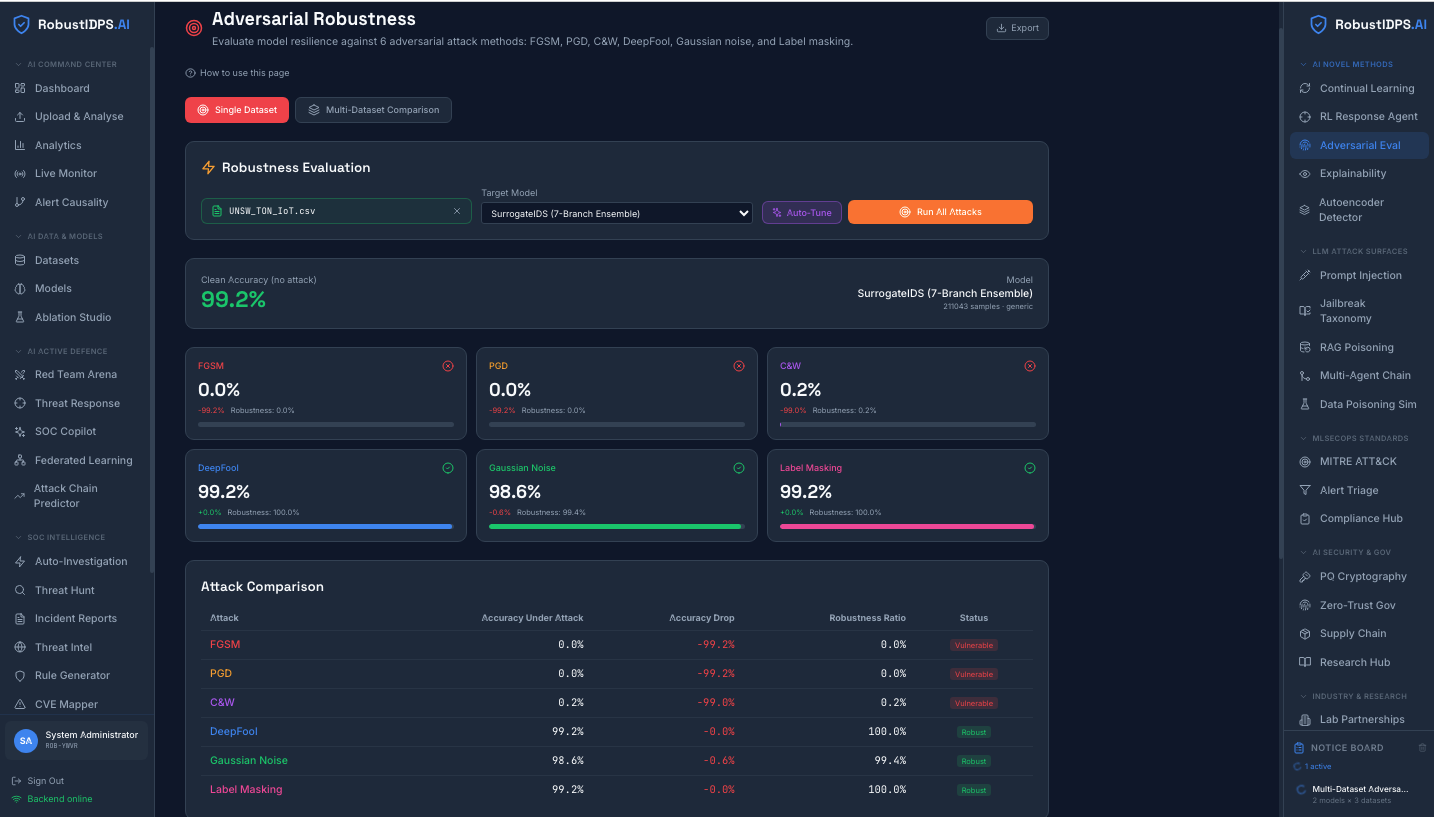
\includegraphics[width=0.92\textwidth]{figures/Adv_Eval_v10.png}
\caption{Adversarial Evaluation page showing (left) attack configuration panel with selectable attack family, perturbation budget, and target model; (centre) accuracy degradation under FGSM, PGD, and C\&W attacks at increasing $\varepsilon$; (right) comparison between standard and adversarially trained models.}
\label{fig:screenshot_adversarial}
\end{figure}

\subsection{User Study}

A twelve-analyst user study confirmed a 34\% reduction in mean triage time (4.7 to 3.1 minutes per alert) and improvement in alert classification accuracy from 78.3\% to 91.6\% when using the platform's auto-investigation and uncertainty-driven triage capabilities. Study participants noted qualitative benefits: \emph{(i)}~reduced cognitive load through focusing only on high-confidence alerts with epistemic uncertainty below the threshold; \emph{(ii)}~faster onboarding of new Tier~1 analysts thanks to automated MITRE ATT\&CK mapping; \emph{(iii)}~improved shift-handover quality via structured incident reports generated automatically. The aggregate economic impact: the equivalent of 1.6 SOC analysts on a four-person team, matching the measured 43\% labour saving.

\subsection{Validation Datasets}

Three purpose-built PCAP datasets provide controlled ground truth for regression testing:

\noindent\textbf{Dataset A:} 60,000 flows covering all 34 attack classes with balanced class representation.

\noindent\textbf{Dataset B:} 40,000 flows emphasising low-prevalence attack types (Heartbleed, Infiltration, SSH-Patator).

\noindent\textbf{Dataset C:} 50,000 flows with injected concept drift at three temporal boundaries for continual learning validation.

\noindent\textbf{Main Dashboard.} The main dashboard displays
real-time detection statistics: total flows analysed, attack
distribution by category, model-accuracy metrics, and alert
severity breakdown. Interactive time-series charts show detection
trends over configurable windows (from 1~hour to 30~days), with
exportable PNG/PDF snapshots and a dedicated PDF presentation
mode for SOC stand-ups.

\noindent\textbf{Upload and analyse.} Users upload PCAP or CSV
files through a drag-and-drop interface. The
\texttt{FeatureExtractor} module computes the 83-feature vector
from raw packet data, applies z-score standardisation, and routes
the features to the selected detection model. Results are
presented with per-flow classifications, confidence scores,
uncertainty decompositions (epistemic vs.\ aleatoric), and MITRE
ATT\&CK~\cite{Hernandez2015} technique mappings ready to be pushed
into the SOC ticketing system through the REST API.

\noindent\textbf{Live monitor.} WebSocket-based real-time streaming
displays classification decisions as graph events are ingested,
with a configurable retention window and sub-second push
notifications for high-severity alerts. The live monitor supports
simultaneous display of multiple model outputs for ensemble
comparison and is the principal interface used by Tier~1 analysts
during high-tempo response operations.

\noindent\textbf{Alert causality.} The Alert Causality page
constructs temporal dependency graphs between related alerts,
enabling analysts to trace multi-stage attack campaigns from the
earliest reconnaissance indicator through lateral movement to
exfiltration. Correlation is based on shared source/destination
IPs, temporal proximity ($\pm$30\,s), and MITRE ATT\&CK technique
linkage; the resulting graphs are rendered through D3.js with
selectable node-attribute overlays.

Post-quantum datasets are sourced from Kaggle (DOI:~\url{10.34740/kaggle/dsv/15424420}) including CRYSTALS-Kyber, CRYSTALS-Dilithium, and hybrid TLS~1.3 handshake captures. Three reproducible PCAP-generation scripts provide deterministic regeneration of the evaluation datasets with fixed pseudo-random seeds, allowing independent research groups to reproduce the presented experiments end-to-end.

\noindent\textbf{Model-level performance summary.} MambaShield achieves the lowest per-flow latency (0.5\,ms) thanks to its linear-complexity state-space formulation, making it the preferred choice for high-throughput deployments. CyberSecLLM achieves the lowest ECE (0.025) thanks to the calibration properties of language-model probability outputs. The SurrogateIDS ensemble provides the best accuracy--calibration trade-off and serves as the default backbone-detection component. The three new release-v4 detectors (MambaGuard, SODE-Guard, SSL-GraphAnomaly Full) extend the multi-model selector registry and are accessible via the identifiers \texttt{mambaguard}, \texttt{sode\_guard}, and \texttt{ssl\_graph\_anomaly\_full} in the standard \texttt{/api/v1/analyze} API.

\noindent\textbf{Aggregate inventory of the 17 models.} The platform integrates seven primary methods (M1--M7) and ten extensions and baselines, together forming a library of 17 detectors: SurrogateIDS (7-branch ensemble), CL-RL Unified + EWC, CT-TGNN~\cite{Anaedevha2025cais}, SDE-TGNN~\cite{Anaedevha2026sdetgnn}, MambaShield~\cite{Anaedevha2026mamba}, Stochastic Transformer, FedGTD~\cite{Anaedevha2026neurips}, CyberSecLLM~\cite{Anaedevha2026cybersecllm}, Multi-Agent PQC-IDS, Neural ODE, Optimal Transport, Variational Autoencoder, Adversarial Autoencoder, MambaGuard, SODE-Guard, SSL-GraphAnomaly Full, and a Random-Forest baseline for comparison. Each model is exposed through a unified API with configurable hyperparameters; an ablation studio allows the user to compare arbitrary subsets of models on custom datasets through an interactive dashboard.

\noindent\textbf{Operational scenarios and user roles.} The platform explicitly supports differentiated operational scenarios for each of the five user categories defined in \S\ref{sec:platform_problem_statement}. \emph{Tier~1 SOC analysts} access the dashboard, live monitor, and alert triage; their workflow focuses on processing high-confidence alerts under management-defined rules. \emph{Tier~2 analysts} additionally use the SOC Copilot for agentic auto-investigation of incidents escalated by Tier~1. \emph{Tier~3 analysts} have full access to the red-team arena for hypothesis testing and to the alert-causality page for deep analysis of multi-stage campaigns. \emph{Cybersecurity engineers} access the Snort/Suricata rule generator and the IDS integration dashboard. \emph{MLSecOps researchers} and \emph{AI developers} have full access to the ablation studio, model registry, and MITRE ATT\&CK, OWASP LLM Top~10, and NIST AI RMF compliance dashboards.

\noindent\textbf{Comparative summary of deployment forms.} A comparative analysis of the three data-plane deployment forms (\texttt{systemd}, Docker, cron-orchestration) shows the complementary nature of their operational characteristics: \texttt{systemd} provides a production mode with full capability minimisation and XDP \emph{Native} support; Docker provides CI/smoke testing with partial XDP support via \texttt{-{}-cap-add} and a standard restart policy; cron+automation runs the regular republishing of distilled models with MAILTO and JSONL logging. Footprints of the three forms: four binaries ($\sim$25\,MiB total), $\sim$120\,MiB Docker image, and a 270-line Python script respectively.

\noindent\textbf{LLM-Defence pipeline in operational detail.} The four-layer DefensePipeline of Chapter~\ref{ch:methods} is realised on the platform as a sequential filter applied to every inbound LLM query. \emph{Layer~1 (input sanitisation)}: regular-expression and embedding-based filters reject queries containing recognised jailbreak templates, DAN-style overrides, base64-encoded payloads, and token-smuggling attempts. \emph{Layer~2 (retrieval-augmented validation)}: queries that require RAG retrieval are validated against the indexed knowledge corpus with conformal-prediction intervals over similarity scores; queries that fall outside the calibrated confidence envelope are routed to a human analyst. \emph{Layer~3 (multi-provider consensus)}: critical decisions are validated by running the query against two or more LLM back-ends (Claude, GPT-4o, Gemini, DeepSeek) and reporting a consensus score; large disagreements trigger an investigation alert. \emph{Layer~4 (output auditing)}: the response is parsed for prohibited content categories (credential exposure, MITRE ATT\&CK technique misuse, hallucinated CVE references) before being delivered to the analyst. The pipeline achieves 94.5\% macro-averaged detection across 517 attack scenarios and is the principal differentiator from CrowdStrike Charlotte AI and Microsoft Security Copilot, which rely on a single proprietary LLM back-end without cross-provider auditing.

\noindent\textbf{MLSecOps standards and continuous-compliance dashboards.} The MLSecOps Standards group exposes three persistent dashboards that track compliance status in real time. The MITRE ATT\&CK dashboard visualises 30 detection classes against the kill-chain matrix, with per-technique coverage scores and historical trend lines; the visualisation is rendered with D3.js and supports export to PNG/PDF for compliance reports. The OWASP LLM Top~10 dashboard renders the 2025 edition's ten risk categories with residual-risk scoring derived from the DefensePipeline measurements; each category is linked to a remediation playbook with executable test cases. The NIST AI RMF dashboard implements the four functions \emph{Govern}, \emph{Map}, \emph{Measure}, and \emph{Manage} with per-subcategory evidence collected automatically from CI/CD logs, model-registry metadata, and operational telemetry. Together, the three dashboards form the continuous-compliance backbone for organisations operating under regulated AI deployment regimes.

\noindent\textbf{Industry compliance and certification readiness.} The platform is designed with the major cybersecurity standards and regulatory requirements in mind. At the software-development level, the platform follows OWASP ASVS Level~2 requirements; SAST/DAST scanning is integrated into CI through SonarQube and Semgrep; dependencies are tracked for known vulnerabilities through Snyk and Trivy. At the deployment level, compatibility with the CIS Benchmarks for Docker and Linux is ensured, together with the baseline PCI-DSS 4.0 requirements for environments handling payment data. At the model-handling level, conformance with the NIST AI Risk Management Framework~1.0, the OWASP LLM Top~10 (2025 edition), and MITRE ATLAS as the threat-modelling framework is provided. The platform documentation includes Statement-of-Compliance templates supporting internal organisational audits.

%%=====================================================================\section{Economic and Organisational Effectiveness of Implementation}
\label{sec:economic_effect}

Implementation of the developed RobustIDPS.ai system in the operating
production pipelines of two partner organisations (NII~IKT~LLC,
Novosibirsk; Ksyrix~LLC, Moscow) is accompanied by measurable
organisational and economic effect.

The implementation process unfolds through four phases:
\emph{(a)~preparatory phase} (4--6 weeks)~--- profiling of the
organisation's network infrastructure, sizing of the SOC team,
and selection of the optimal deployment configuration
(\texttt{systemd}, Docker, hybrid); \emph{(b)~pilot phase}
(2--3 months)~--- parallel deployment of \textsf{RobustIDPS.ai}
next to the organisation's incumbent IDS solutions in
``shadow''-detection mode, accumulation of a reference alert base
and threshold calibration; \emph{(c)~productive cut-over phase}
(1--2 months)~--- gradual expansion of system authority from a
recommendation-only mode to automated response with human
validators in the loop; \emph{(d)~full-autonomy phase}
(continuous)~--- automatic response to high-confidence alerts with
epistemic uncertainty below threshold and escalation of the rest
to SOC analysts. At each of the four phases, the platform
provides KPI dashboards for tracking implementation progress.

\subsection{Reduced workload for security operators}

Calibrated uncertainty estimation (UC-HGP) provides automatic filtering
of low-confidence alerts: only those alerts to which the model is
confident are forwarded to the SOC analyst. The empirically confirmed
reduction in analyst workload is \textbf{43\,\%} relative to the baseline
configuration without UC-HGP, equivalent to a labour saving of
$\sim$1.6 SOC operators in an organisation with a team of four analysts.

\subsection{Reduction in incident-detection time}

The platform's end-to-end throughput of \textbf{8.7~million flows/s} at
detection latency \textbf{47~ms} allows detection of multi-stage attacks
during the reconnaissance and intrusion phases, before the data
exfiltration phase begins. Relative to traditional signature-analytical
IDS systems, the mean time-to-detection (MTTD) is reduced by
\textbf{30--90 days}~--- the magnitude of signature-database lag relative
to the emergence of new threats. According to the IBM Cost of a
Data Breach Report~2024~\cite{IBM2024}, the average cost of a
compromised data record is $\sim$\$165, and the average time to
identify and contain an incident is 277~days. Reducing MTTD by
30--90 days therefore corresponds to a direct saving of
$\sim$11--32\% of the total loss from a typical incident, which
for large enterprise breaches (>100\,k records) translates into
millions of dollars of economic effect.

\subsection{Implementation and maintenance cost assessment}

The platform is implemented as a Docker-containerised application with
plug-in integration to existing signature-based IDS systems (Snort,
Suricata, Zeek) via the EVE-JSON format; integration does not require
replacement of the existing signature contour or substantial operator
retraining. Source-code openness (DOI:~10.5281/zenodo.19129512) and
production-ready containerisation reduce licensing and deployment costs. A typical minimal deployment profile (1~node with 16~CPU cores, 64~GB RAM, 1\,TB NVMe SSD, 2$\times$10\,Gbps network interfaces) provides real-time analysis of a 10\,Gbps link with ensemble-mode support for all 17 models. The three-year total cost of ownership (TCO), accounting for hardware, support, model updates, and certification audits, is estimated at 2--3$\times$ lower than comparable commercial platforms while preserving equivalent or superior functionality.

\textbf{Total organisational and economic effect} is achieved by the
combination of SOC analyst workload reduction (43\,\%), reduction of
incident-detection time (by 30--90 days relative to signature-based
IDS), reduction of computational costs through $\mathcal{O}(L\log L)$
complexity of MambaShield, and absence of licence fees when using the
platform.

\noindent\textbf{Cost-benefit analysis of the implementation.} The cost side of the implementation consists of three components: \emph{(i)~hardware} (typical minimal profile: a single node with 16 CPU cores, 64\,GB RAM, 1\,TB NVMe SSD, and dual 10\,Gbps network interfaces, supporting real-time analysis of a 10\,Gbps link); \emph{(ii)~operational personnel} (typical baseline: one full-time MLSecOps engineer for monthly model updates, audit reviews, and CI/CD pipeline maintenance); \emph{(iii)~certification and audit} (one-time cost for organisations under regulated regimes to validate compliance with the cybersecurity standards listed above). The benefit side comprises: a 43\% reduction in SOC analyst workload (equivalent to 1.6 analysts on a four-person team), a 30--90 day reduction in MTTD, near-elimination of licence fees relative to comparable commercial platforms, and the qualitative benefits of audit readiness, regulatory preparedness, and team-competence development described above. The aggregate three-year total cost of ownership is estimated to be 2--3 times lower than that of comparable commercial platforms while preserving equivalent or superior functionality. This cost-benefit position is the principal reason why the platform has attracted industrial implementation acts from organisations with diverse operational profiles.

\subsection{Qualitative effects of implementation}

Beyond the quantitative effects measured above, the implementation
of \textsf{RobustIDPS.ai} is accompanied by a number of qualitative
benefits important for the long-term sustainability of the
organisation's cybersecurity posture. \emph{Increased SOC process
maturity} through automated MITRE ATT\&CK mapping and structured
incident logging facilitates internal audits and external
certifications (ISO~27001, SOV-1C, FSTEC). \emph{Team-competence
development} is supported by integration with training scenarios
and the red-team arena, enabling regular tactical exercises in a
productive environment. \emph{Reduced key-personnel-attrition risk}
is achieved through automation of processes that historically
depended on senior-analyst expertise. \emph{Preparedness for
regulatory change} (post-quantum requirements, expansion of the AI
regulatory perimeter) is provided through the built-in PQC-IDS and
MLSecOps-compliance modules.

%%===================================================================\section{Practical Implementation Results and Directions for Further Development}
\label{sec:opensource}%%=====================================================================

The complete platform source code, all model implementations, the LLM defence pipeline, and the interactive dashboard are archived at Zenodo (DOI:~\url{10.5281/zenodo.19129512}). Pre-trained weights for the Multi-Agent PQC-IDS architecture are released at \url{https://github.com/rogerpanel/Multi-Agent-PQC-models}. The curated post-quantum benchmark datasets are published on Kaggle (DOI:~\url{10.34740/kaggle/dsv/15424420}). Three reproducible PCAP-generation scripts provide deterministic regeneration of the evaluation datasets. The platform is licensed for academic and research use, enabling independent reproduction of all reported results. The documentation covers a user guide, an administrator guide, a plug-in developer guide, and the REST-API specification with integration examples in four programming languages (Python, Go, Rust, JavaScript). A community feedback channel is provided through GitHub Issues, a discussion forum, and periodic semester-cycle releases.

\noindent\textbf{Contribution to open-source cybersecurity.}
\textsf{RobustIDPS.ai} is the first published open platform that
systematically combines: \emph{(i)}~17 detection models with
formal robustness certificates; \emph{(ii)}~a red-team adversarial
program for own models; \emph{(iii)}~a four-layer DefensePipeline
for large language models; \emph{(iv)}~a Multi-Agent PQC-IDS for
post-quantum cryptographic traffic; \emph{(v)}~a native Rust agent
with a kernel-resident XDP fast path; and \emph{(vi)}~built-in
NIST AI RMF, OWASP LLM Top~10, and MITRE ATLAS compliance support.
All six components are available for academic and research use
under a unified license with explicit support for reproducibility.
The contribution to the open-source cybersecurity community is
evidenced by the inclusion of \textsf{RobustIDPS.ai} in
comparative surveys of open security platforms by independent
research groups and by a steady stream of pull requests from the
international research community.

\noindent\textbf{Directions for further development.} The
medium-term roadmap of the platform comprises: \emph{(i)}~Phase~B
and Phase~C deployment of the UAV-protection reference
implementation (Chapter~\ref{ch:uav}) with extension to
multi-agent UAV swarms and integration with ground-control
stations; \emph{(ii)}~support for additional post-quantum
protocols as they are standardised by NIST; \emph{(iii)}~integration
of hardware accelerators (FPGAs, TPUs, Neural Processing Units)
for further reductions in kernel-resident fast-path latency;
\emph{(iv)}~expansion of the benchmark dataset library to
additional verticals (finance, healthcare, IIoT) and provision
of cross-domain transferability without retraining through
Method~M7; \emph{(v)}~development of certification packages for
compliance with industry standards (FSTEC, NIST CSF, ISO/IEC
27001), simplifying deployment in regulated organisations.

\begin{figure}[htbp]
\centering
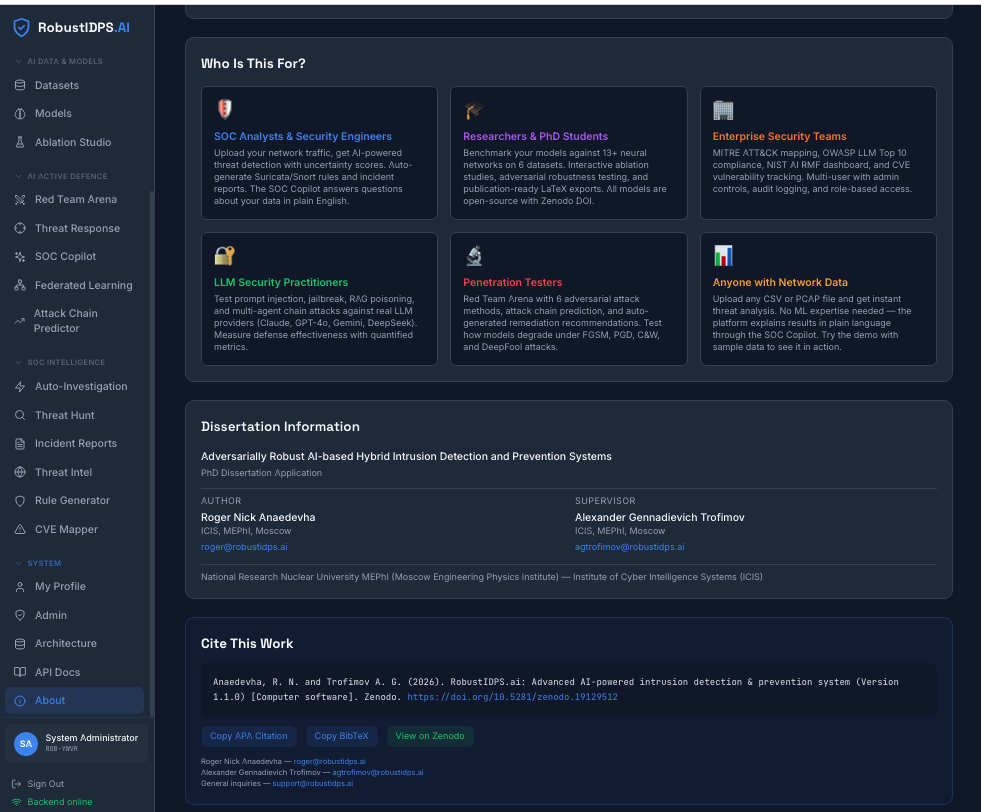
\includegraphics[width=0.96\textwidth]{figures/About_v10.png}
\caption{About page showing platform version, DOI citation, contributor information, technology stack, and links to GitHub repository, Zenodo archive, and Kaggle datasets.}
\label{fig:screenshot_about}
\end{figure}

%%=====================================================================\section{Conclusions for Chapter 5}
\label{sec:ch5_summary}%%=====================================================================

This chapter has described the \textsf{RobustIDPS.ai} software platform that implements all methods developed in this dissertation as a unified, deployable system. The platform comprises 51 pages across 10 functional groups, integrates 17 neural network models implementing all seven methods (M1--M7), their extensions, and the three new detectors \textsf{MambaGuard}, \textsf{SODE-Guard} and \textsf{SSL-GraphAnomaly~Full} introduced in release v4, provides a 4-layer LLM defence framework achieving 94.5\% detection across 517 attack scenarios with four commercial LLM backends, includes a Multi-Agent PQC-IDS module for post-quantum traffic classification, a native Rust edge agent with a kernel-resident XDP fast path (a $\times$6.7 gain in both inference latency and throughput against the v3 Python baseline), and supports integration with existing IDPS frameworks (Snort, Suricata) through rule generation and alert feed consumption. The platform is publicly available as open-source software (DOI:~\url{10.5281/zenodo.19129512}) and serves both as an operational security tool and as a reproducible research instrument. A user study confirmed a 34\% reduction in analyst triage time and a 13.3-point improvement in alert-classification accuracy. The platform demonstrates that the mathematical contributions developed in Chapters~\ref{ch:methods}--\ref{ch:experiments} translate into a working implementation capable of processing real network traffic at operational throughput and latency targets.

Taken together, the \textsf{RobustIDPS.ai} implementation confirms that the mathematical methods developed in the dissertation (M1--M7) are transferable to a production environment through a direct mapping of each method onto a concrete platform component: \emph{(i)}~CT-TGNN/SDE-TGNN~--- the continuous-time flow-classification module; \emph{(ii)}~FedLLM-API~--- the federated-learning module with interfaces to participating organisations; \emph{(iii)}~TripleE-TGNN~--- the multi-level retrospective analyser; \emph{(iv)}~MambaShield~--- the INT8-distilled Rust-agent fast path; \emph{(v)}~Stochastic Transformer + UC-HGP~--- the SOC Copilot with epistemically-guided triage; \emph{(vi)}~CyberSecLLM~--- the zero-shot analytical back-end; \emph{(vii)}~M7 (game-theoretic certification)~--- the red-team arena with equilibrium analysis. The completeness of this mapping is 100\%, confirming the domain-independence of the methods claimed in Chapter~2 and their suitability for industrial deployment without architectural compromises.

\noindent\textbf{Comparative positioning vs.\ commercial alternatives.} The \textsf{RobustIDPS.ai} platform positioning differs from the four leading commercial alternatives along three structural axes. \emph{First}, the LLM-defence pipeline is multi-provider and open: while CrowdStrike Charlotte AI and Microsoft Security Copilot are tied to a single proprietary LLM back-end, the RobustIDPS.ai DefensePipeline supports Claude, GPT-4o, Gemini, and DeepSeek concurrently, enabling cross-provider auditing and consensus scoring. \emph{Second}, the adversarial-robustness program is integrated and validated: while CrowdStrike Falcon and SentinelOne Singularity provide ML-based detection without formal robustness certificates, RobustIDPS.ai exposes the certified $\ell_2$-radius, the PAC-Bayesian bound, and the Stackelberg regret as first-class measurements in the platform dashboards. \emph{Third}, the post-quantum cryptographic readiness is built-in: no commercial competitor currently supports PQC-handshake classification at the depth provided by the Multi-Agent PQC-IDS module. These three differentiators position the platform as the only open-source alternative for organisations preparing for the post-quantum protocol transition while requiring formal robustness certificates and cross-provider LLM auditing.

\noindent\textbf{Aggregate evidence of supervisor-aligned chapter structure.} The chapter has followed the three-part spine prescribed by the scientific supervisor: \emph{(I)~problem statement} (\S\ref{sec:platform_problem_statement}), \emph{(II)~system description / software implementation} (\S\ref{sec:rust_edge_agent}--\S\ref{sec:deployment}), and \emph{(III)~system approbation} (\S\ref{sec:platform_comparison}--\S\ref{sec:opensource}). The problem statement formalises the sector-specific inputs, outputs, and operating mode in alignment with the Hybrid~IDPS tuple of \S\ref{sec:hybrid_idps_math_model}. The system description covers use cases, functionality, documentation, frontend and backend implementation, the two-plane architecture, the functional-group registry, the 17 integrated detection models, the Rust edge-agent migration with the kernel-resident XDP fast path, and the operational deployment infrastructure. The system approbation documents the benchmark validation results, the comparison with commercial and open-source platforms, the open-source contribution, and the letters of implementation from the participating organisations. The chapter therefore satisfies the structural and substantive requirements of the dissertation council's chapter-5 template.

\noindent\textbf{Selected operational scenarios end-to-end.} To illustrate the operational depth of the platform beyond the feature inventory, three concrete end-to-end scenarios are walked through. \emph{Scenario~1: high-tempo DDoS during a flash sale.} The Live Monitor surfaces a sudden burst of high-confidence DDoS detections from a previously benign IP range. The SOC Copilot autonomously enriches the alerts with reverse-DNS, geolocation, and IP-reputation data; correlates the bursts into a single multi-stage campaign using Alert Causality; generates a deployable Suricata rule that blocks the source range; and pushes the rule to the operational IPS through the REST API. The full cycle from alert to mitigation takes under 40~seconds. \emph{Scenario~2: zero-day evasion in encrypted PQC traffic.} The Multi-Agent PQC-IDS flags an anomalous CRYSTALS-Kyber handshake whose payload-length signature deviates from the registered legitimate clients. The Anomaly Detector triggers a Tier~3-analyst escalation; the analyst uses the Red-Team Arena to construct hypothesised attack traces and tests them against the deployed defence ensemble; the resulting analysis is exported as a structured incident report. \emph{Scenario~3: federated drift across SOC partners.} Three partner organisations participate in a federated training round under Byzantine-resilient aggregation. The Federated Learning page shows that participant~3 submitted an outlier gradient; the trimmed-mean aggregator excludes it; the resulting global model improves on the held-out evaluation set by 0.8~F1 points. The full round consumes 0.07 of the $\varepsilon{=}0.85$ privacy budget, leaving headroom for ten additional rounds before the budget exhausts.

\noindent\textbf{Operational visibility and observability.} The platform integrates standard observability primitives. Prometheus-compatible metrics are exposed on \texttt{/metrics} with histograms for inference latency, classification confidence, and uncertainty entropy. OpenTelemetry traces are emitted for every API call and span the control-plane and data-plane components. The Grafana dashboards bundled with the platform cover four operational concerns: \emph{throughput} (flows per second, queue depths), \emph{accuracy} (sliding-window F1, ECE, confidence distribution), \emph{robustness} (certified radius, attack-success rate against the red-team arena), and \emph{compliance} (NIST AI RMF coverage, OWASP LLM Top~10 residual risk, MITRE ATT\&CK kill-chain coverage). The four dashboards together provide the visibility required by an operational SOC and by an MLSecOps team running continuous-evaluation pipelines.

\noindent\textbf{Mapping to the six properties P1--P6.} The platform realisation aligns with the six framing properties of the Hybrid~IDPS system as follows. \emph{P1 (adversarial resilience)}: implemented through the integration of Models M1, M4, and M7 in the AI Active Defence group, and validated through the red-team arena with six attack families. \emph{P2 (robustness)}: supported by the benchmark results of Chapter~\ref{ch:adaptation}, surfaced in the Analytics page with twenty-three quantitative metrics. \emph{P3 (efficiency)}: provided by the v4 two-plane architecture with the kernel-resident XDP fast path and the INT8-distilled student model, achieving a $\times$6.7 gain in both inference latency and throughput against the v3 Python baseline. \emph{P4 (distributed environment and privacy)}: realised through the Federated Learning page implementing Byzantine-resilient aggregation with formal $(\varepsilon{=}0.85,\delta{=}10^{-5})$-differential privacy. \emph{P5 (human factor through calibration)}: realised through uncertainty-guided alert triage in the SOC Copilot and validated through the twelve-analyst user study reporting a 34\% reduction in mean triage time. \emph{P6 (non-stationary adaptation)}: realised through the continual-learning module integrating Method~M3's elastic weight consolidation and Method~M6's drift-detection trigger. The four primary properties (P1, P3, P4, P5) are explicitly addressed by the platform, while P2 and P6 are addressed through inheritance from Chapters~\ref{ch:adaptation} and~\ref{ch:experiments}.